\section{Metodologie utilizzate}

\subsection{Studio del problema}
Lo \textbf{spam} è l'invio anche verso indirizzi generici, non verificati o sconosciuti, di messaggi ripetuti ad alta frequenza o a carattere di monotematicità tale da renderli indesiderati. Il problema dello spam nasce quando, con l'avvento di tecnologie informatiche, questa tipologia di messaggi ha iniziato ad invadere le caselle di posta elettronica e gli smartphone di aziende e semplici utilizzatori. Ciò ha portato molte persone ad interessarsi al tema dello spam e di come riuscire a contrastarlo in modo efficace.
\newline
In prima battuta, ci sono state molte discussioni riguardanti la tipologia del problema. Le principali controversie furono tra chi sosteneva fosse un problema di \textit{classificazione} e tra chi, invece, sosteneva fosse un problema di \textit{modellazione}.
Alcune correnti di pensiero continuano a sostenere che la metodologia migliore da applicare in questo caso sia la modellazione, ma la maggior parte della comunità degli studiosi afferma con convinzione che la tecnica migliore sia quella della classificazione. Noi concordiamo con quest'ultimi, vero che il bisogno iniziale di dati già classificati è uno svantaggio, ma nell'era dei big data, è ormai semplice trovare dei set di dati consistenti e pronti all'uso. Inoltre, c'è da sottolineare la maggiore flessibilità della tecnica che è portata maggiormente ad imparare dai propri errori.
\newline
Detto ciò, si può capire perché tra i tanti tipi di approcci al problema abbiamo deciso di utilizzare la \textit{Logistic Regression} e le \textit{Neural Networks}, vediamoli ora in modo più approfondito.
\subsection{Neural networks}
Le \href{https://en.wikipedia.org/wiki/Neural_network}{Neural networks}, o reti neurali, sono ispirate alle reti di neuroni biologici. Solitamente, sono sistemi che imparano dagli esempi e che inizialmente sono configurati in modo randomizzato.\\
Il concetto alla base è il singolo neurone artificiale, che poi viene rappresentato in collezioni connesse con altri neuroni, come nelle reti biologiche.

\begin{figure}[H]
\centering
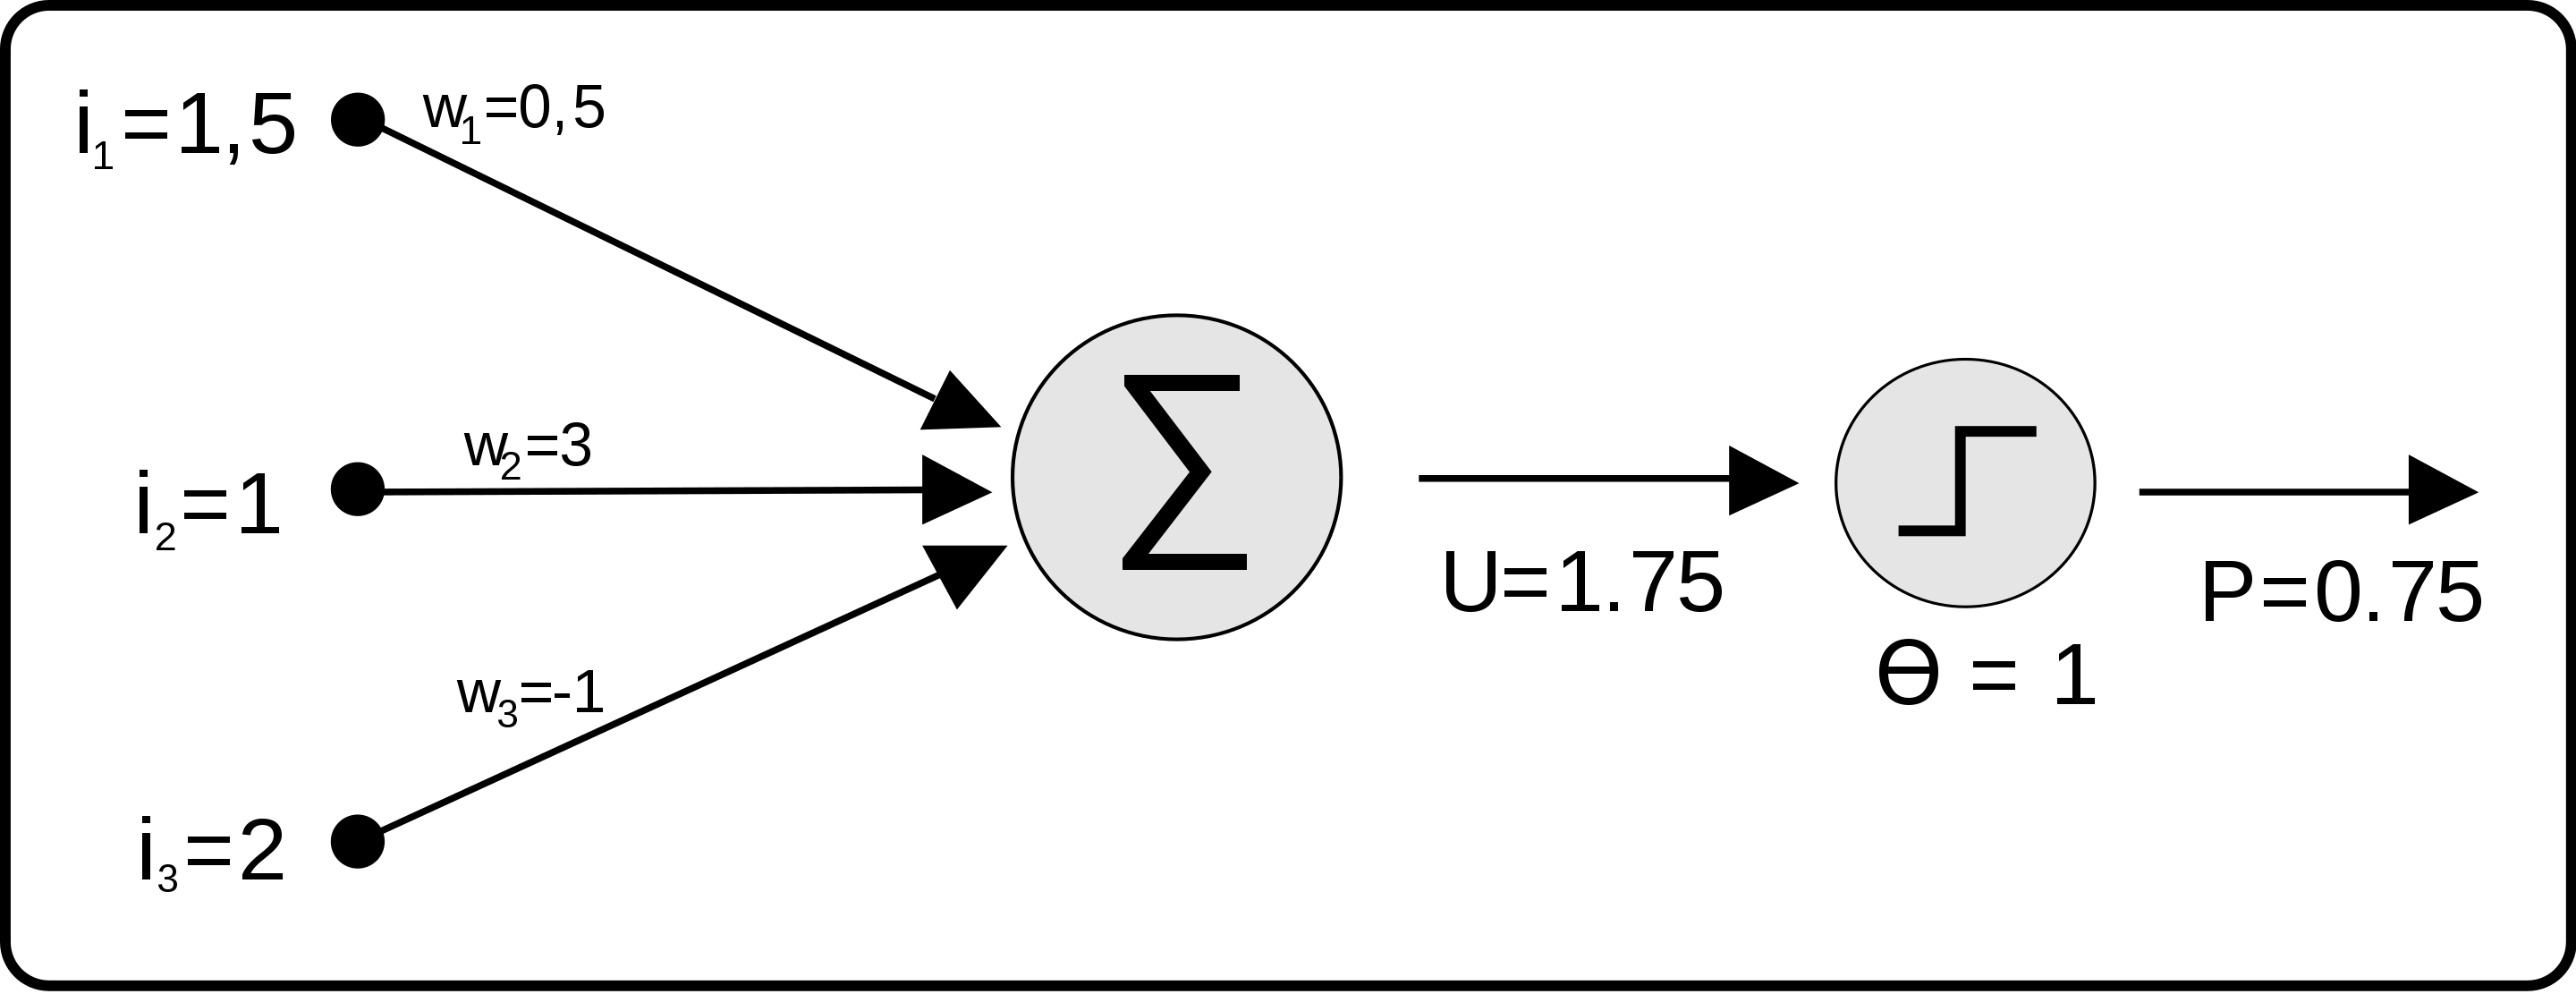
\includegraphics[scale=0.1]{img/neuroneArtificiale.png}
\caption{Esempio di neurone artificiale}
\end{figure}

Queste collezioni vengono comunemente chiamati layer e le connessioni tra ogni nodo vengono chiamati edge.\\
Ad ogni neurone e ad ogni edge viene assegnato un peso, il quale, in concreto, ha la funzione di "aggiustamento" del tasso di apprendimento influenzando la il valore dei nodi o delle connessioni.

\subsection{Logistic Regression}
La \href{https://en.wikipedia.org/wiki/Logistic_regression}{Logistic Regression}  è un modello statistico che si basa sull'utilizzo della Logistic Function per modellare una variabile binaria dipendente.
\begin{equation}
\sigma (t)={\frac {e^{t}}{e^{t}+1}}={\frac {1}{1+e^{-t}}}
\end{equation}
Il fulcro della Logistic Regression sta nell'assegnare un valore che va da 0 a 1 della probabilità che un dato elemento sia o meno del tipo A, ovviamente la somma delle probabilità di appartenere o del non appartenere alla categoria A deve essere esattamente 1. Sottolineiamo quindi che, come dal nome, è una forma di regressione matematica.\\ Interessante la possibilità di avere un grado maggiore o minore di tolleranza, e quindi una sorta di scelta, spostando in alto o in basso la soglia minima per essere considerati di un certo tipo. Questo ci consente maggiore flessibilità in caso di incertezza del nostro algoritmo o maggiore rigidezza in caso di estrema precisione.
\begin{figure}[H]
\centering
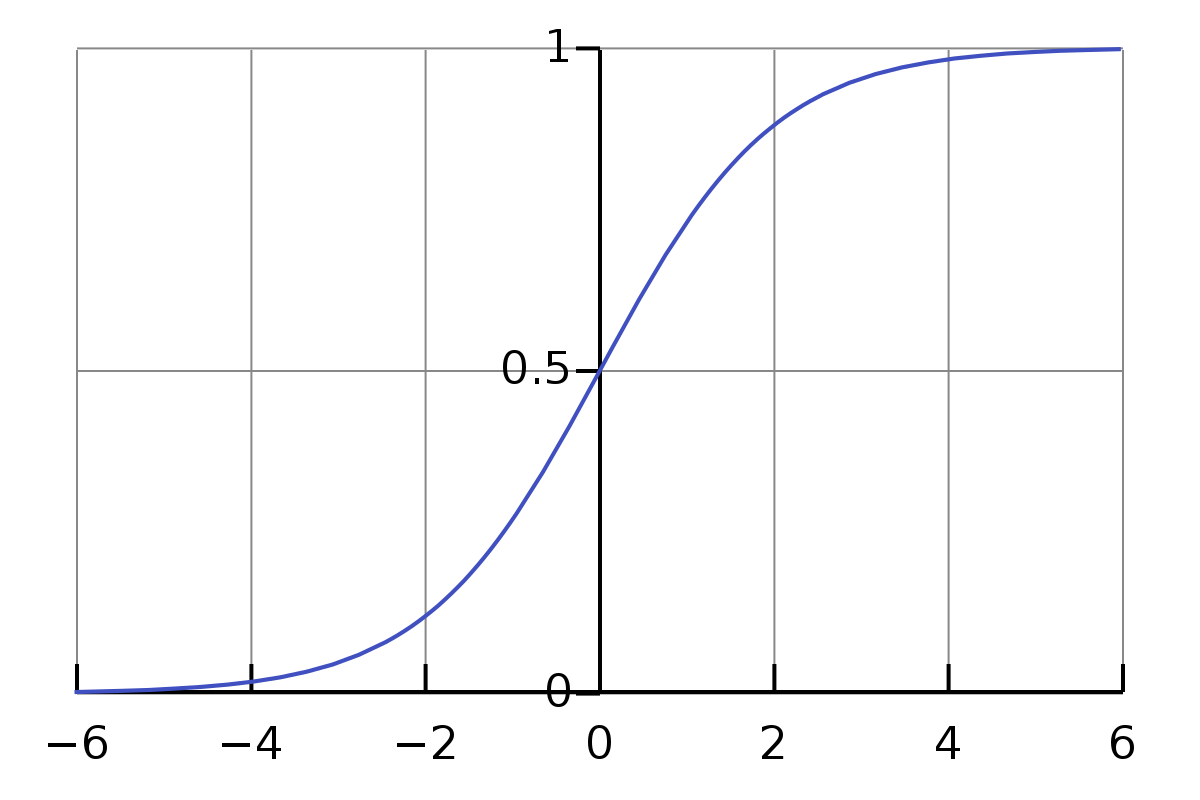
\includegraphics[scale=0.25]{img/logisticFunction.png}
\caption{La logistic function standard}
\end{figure}
